%!TEX root = ../ICR.tex
\chapter{Metodología \label{cap:Metodologia}}

En este capítulo se detalla el procedimiento experimental seguido para abordar el problema de la detección de noticias falsas en español. La metodología se diseñó con un enfoque evolutivo y comparativo, comenzando con una exploración de técnicas de optimización clásicas y culminando con la implementación de un modelo de lenguaje de última generación. El diseño del flujo de trabajo, ilustrado en la Figura \ref{fig:metodologia_general}, garantiza la reproducibilidad de los resultados al definir claramente cada una de sus etapas, desde la recopilación de datos hasta la evaluación final y la implementación de una aplicación web como solución práctica.

\section{Visión General de la Metodología}

La estrategia metodológica de esta tesis se fundamenta en la comparación sistemática de dos paradigmas de la inteligencia artificial sobre un corpus unificado de gran escala. Como se muestra en la Figura \ref{fig:metodologia_general}, ambos enfoques parten de una base común (la problemática y los datos), pero siguen rutas de implementación y modelado distintas, para finalmente ser evaluados bajo un mismo marco de métricas y así determinar la solución más eficaz que será implementada en una aplicación web.

El primer paradigma se basa en técnicas clásicas de Procesamiento del Lenguaje Natural (PLN) con representación Bolsa de Palabras (BoW) y optimización metaheurística, mientras que el segundo emplea modelos Transformer pre-entrenados con técnicas de fine-tuning. Esta aproximación comparativa permite evaluar tanto la efectividad como la eficiencia computacional de cada enfoque en el contexto específico de la detección de desinformación en español.

Una vez determinado el mejor modelo mediante las métricas de evaluación correspondientes, se procederá a desarrollar una aplicación web funcional que permita la detección automática de noticias falsas en tiempo real.

\begin{figure}[h!]
    \centering
    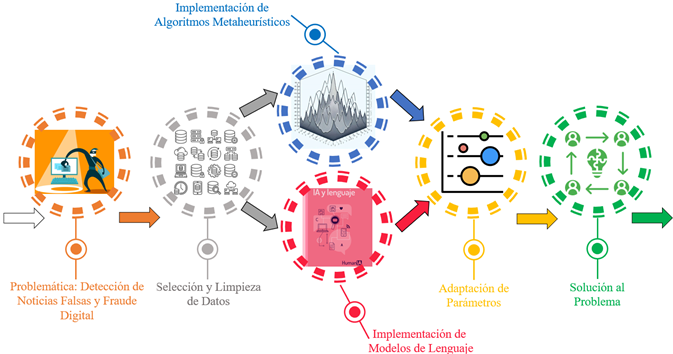
\includegraphics[width=\textwidth]{Imagenes/metodologiaCompleta.png}
    \caption{Metodología propuesta que aborda la problemática combinando Algoritmos Metaheurísticos y Modelos de Lenguaje.}
    \label{fig:metodologia_general}
\end{figure}

\section{Definición y Distinción de Conceptos Fundamentales}
\label{sec:definicion_conceptos}

Antes de proceder con la descripción metodológica, es fundamental establecer con precisión la terminología utilizada en esta investigación, particularmente la distinción entre conceptos relacionados pero diferenciados que a menudo se utilizan de manera intercambiable en la literatura.

\subsection{Distinción entre Noticia Falsa y Bulo}

En el contexto de esta investigación, es esencial distinguir entre dos conceptos fundamentales que, aunque relacionados, poseen características distintivas importantes para el desarrollo de sistemas de detección automática.

% Definir colores adicionales para las tablas de conceptos
\definecolor{LightGreen}{RGB}{144, 238, 144}
\definecolor{LightCoral}{RGB}{240, 128, 128}
\definecolor{LightSkyBlue}{RGB}{135, 206, 250}
\definecolor{LightGoldenrod}{RGB}{250, 250, 210}
\definecolor{LightPink}{RGB}{255, 182, 193}


\subsection{Taxonomía de la Desinformación}

Para proporcionar un marco conceptual completo, esta investigación adopta la taxonomía establecida por la literatura internacional \cite{bondielli2019survey, hu2022deep}, que clasifica el contenido engañoso en tres categorías principales:

\begin{enumerate}
    \item \textbf{\gls{desinformacion}}: Información falsa creada y compartida deliberadamente con intención maliciosa
    \item \textbf{\gls{misinformacion}}: Información incorrecta compartida sin intención maliciosa
    \item \textbf{\gls{malinformacion}}: Información genuina compartida con intención de causar daño
\end{enumerate}

El alcance de esta investigación se centra específicamente en la detección automática de \textbf{desinformación}, abarcando tanto noticias falsas como bulos, reconociendo que ambos tipos requieren estrategias de procesamiento de lenguaje natural diferenciadas pero complementarias.

\subsection{Justificación de la Unificación Terminológica}

En el contexto del desarrollo de sistemas automáticos de detección, la distinción entre noticia falsa y bulo, aunque conceptualmente importante, se aborda mediante un enfoque unificado de \textbf{detección de contenido desinformativo}. Esta decisión metodológica se fundamenta en:

\begin{itemize}
    \item \textbf{Características textuales compartidas}: Ambos tipos utilizan patrones lingüísticos identificables mediante técnicas de PLN
    \item \textbf{Objetivo común}: La finalidad de engañar o desinformar a la audiencia
    \item \textbf{Impacto social similar}: Efectos negativos en la percepción pública y toma de decisiones
    \item \textbf{Necesidad práctica}: Los sistemas de detección automática deben ser capaces de identificar ambos tipos
\end{itemize}

Por tanto, en el resto de este documento, el término \textbf{``noticias falsas''} se utilizará de manera inclusiva para referirse a cualquier tipo de contenido desinformativo, reconociendo la diversidad de formatos y estrategias de propagación que abarca esta categorización.

\section{Construcción del Corpus Unificado}
\label{sec:construccion_corpus}

El primer y más fundamental paso de la metodología fue la construcción de un corpus de alta calidad y de tamaño significativo en español, dada la escasez documentada de recursos centralizados para esta tarea \cite{hu2022deep}.

\begin{table}[htbp]
\centering
\adjustbox{width=\textwidth,center}{%
\footnotesize
\begin{tabular}{|c|l|l|c|c|l|c|}
\hline
\rowcolor{UAMPurple!20}
\textbf{Aspecto} & \textbf{Noticia Falsa} & \textbf{Bulo} \\
\hline
\rowcolor{LightGreen!30}
\textbf{Definición} & 
Información deliberadamente fabricada que se presenta como noticia legítima, pero contiene datos falsos, inexactos o engañosos & 
Información falsa que circula ampliamente, especialmente en redes sociales, con propósito de engañar a la audiencia \\
\hline
\rowcolor{LightSkyBlue!30}
\textbf{Formato} & 
Apariencia de contenido periodístico real, formato de noticia tradicional con titular, cuerpo, fecha, fuente & 
No necesariamente formato periodístico, puede ser texto libre, memes, cadenas de WhatsApp \\
\hline
\rowcolor{LightCoral!30}
\textbf{Intención} & 
Intención maliciosa de desinformar simulando legitimidad periodística & 
Propósito de engañar que apela más a emociones que a hechos verificables \\
\hline
\rowcolor{LightGoldenrod!30}
\textbf{Propagación} & 
Se distribuye a través de sitios web que simulan medios legítimos o plataformas de noticias & 
Circulación viral en redes sociales, aplicaciones de mensajería, cadenas de reenvío \\
\hline
\rowcolor{LightPink!30}
\textbf{Ejemplos} & 
Artículos con titular sensacionalista, byline falso, citas inventadas, estadísticas manipuladas & 
Teorías conspirativas, información médica falsa, rumores políticos, cadenas de ``urgente'' \\
\hline
\rowcolor{HeaderBlue!20}
\textbf{Relevancia para PLN} & 
Estructura textual más predecible, patrones estilísticos identificables en el análisis automatizado & 
Variabilidad estructural mayor, requiere análisis semántico y contextual más sofisticado \\
\hline
\end{tabular}
}
\caption{Comparación detallada entre noticia falsa y bulo en el contexto de detección automática.}
\label{tab:noticia_falsa_vs_bulo}
\end{table}



% Definir colores adicionales para hacer las tablas más coloridas
\definecolor{LightGreen}{RGB}{144, 238, 144}
\definecolor{LightCoral}{RGB}{240, 128, 128}
\definecolor{LightSkyBlue}{RGB}{135, 206, 250}
\definecolor{LightGoldenrod}{RGB}{250, 250, 210}
\definecolor{LightPink}{RGB}{255, 182, 193}

\subsection{Fuentes de Datos Académicas}

Se llevó a cabo un proceso exhaustivo de investigación y unificación de cuatro corpus académicos reconocidos, los cuales constituyen pilares en la investigación de noticias falsas en español. La Tabla \ref{tab:corpus_academicos} presenta un resumen detallado de estos recursos.

\begin{table}[htbp]
\centering
\adjustbox{width=\textwidth,center}{%
\footnotesize
\begin{tabular}{|c|l|l|c|c|l|c|}
\hline
\rowcolor{UAMPurple!20}
\textbf{ID} & \textbf{Nombre del Corpus} & \textbf{Autores Principales} & \textbf{Año} & \textbf{Noticias} & \textbf{Características} & \textbf{Ref.} \\
\hline
\rowcolor{LightGreen!30}
1 & \begin{tabular}[t]{@{}l@{}}Spanish Fake News Corpus\\(IberLEF)\end{tabular} & \begin{tabular}[t]{@{}l@{}}Posadas-Durán, J.P.\\Gómez-Adorno, H.\end{tabular} & 2019-2021 & 971 & \begin{tabular}[t]{@{}l@{}}Análisis estilométrico\\Múltiples versiones\end{tabular} & \cite{posadas2019detection} \\
\hline
\rowcolor{LightSkyBlue!30}
2 & \begin{tabular}[t]{@{}l@{}}Dataset Zules Acosta\\(UPM)\end{tabular} & Acosta, F.A.Z. & 2019 & 598 & \begin{tabular}[t]{@{}l@{}}Trabajo fin de máster\\Web scraping verificado\end{tabular} & \cite{acosta2019construccion} \\
\hline
\rowcolor{LightCoral!30}
3 & \begin{tabular}[t]{@{}l@{}}Dataset Tretiakov\\(Kaggle)\end{tabular} & \begin{tabular}[t]{@{}l@{}}Tretiakov, A.\\Martín García, A.\end{tabular} & 2022 & 1,958 & \begin{tabular}[t]{@{}l@{}}Machine Learning\\Disponible públicamente\end{tabular} & \cite{tretiakov2022detection} \\
\hline
\rowcolor{LightGoldenrod!30}
4 & \begin{tabular}[t]{@{}l@{}}Spanish Political Fake News\\Dataset\end{tabular} & \begin{tabular}[t]{@{}l@{}}Blanco-Fernández, Y.\\Otero-Vizoso, J.\end{tabular} & 2024 & 57,231 & \begin{tabular}[t]{@{}l@{}}Temática política\\Modelos BERT/RoBERTa\end{tabular} & \cite{blanco2024enhancing} \\
\hline
\rowcolor{HeaderBlue!20}
\multicolumn{5}{|c|}{\textbf{TOTAL CORPUS ACADÉMICOS}} & \textbf{60,758} & \textbf{Cuatro fuentes} \\
\hline
\end{tabular}
}
\caption{Corpus académicos utilizados para la construcción del dataset unificado.}
\label{tab:corpus_academicos}
\end{table}

\subsubsection{Spanish Fake News Corpus (IberLEF)}

Este corpus, asociado a las competencias de IberLEF y desarrollado por Posadas-Durán, Gómez-Adorno, et al., ha tenido varias versiones. La versión original y más citada del corpus contiene un total de 971 noticias \cite{posadas2019detection}. Este corpus se caracteriza por su enfoque en análisis estilométrico y ha sido utilizado en múltiples evaluaciones comparativas dentro del marco de las competencias IberLEF \cite{gomez2021overview, aragon2020overview}. Las versiones posteriores del corpus han sido mantenidas y actualizadas en repositorios públicos \cite{ramirez2021spanish}.

\subsubsection{Dataset de Zules Acosta (Universidad Politécnica de Madrid)}

Desarrollado como parte de un Trabajo Fin de Máster Universitario en Ciberseguridad en la Universidad Politécnica de Madrid, este corpus contiene 598 noticias verificadas \cite{acosta2019construccion}. El dataset fue construido mediante técnicas de web scraping y se encuentra disponible públicamente en la plataforma Kaggle \cite{acosta2019dataset, zules2019spanish}. Su contribución principal radica en la aplicación de metodologías rigurosas de verificación para la construcción de datasets de noticias falsas.

\subsubsection{Dataset de Tretiakov et al.}

Este corpus, desarrollado por Tretiakov, Martín García y Camacho, contiene 1,958 noticias falsas en español \cite{tretiakov2022detection}. El dataset fue creado en el contexto de técnicas de aprendizaje automático para la detección de información falsa y se encuentra disponible públicamente en Kaggle \cite{tretiakov2022noticias}. Su enfoque se centra en la aplicación de técnicas de machine learning para la clasificación automatizada de contenido desinformativo.

\subsubsection{Spanish Political Fake News Dataset}

El corpus más extenso utilizado, desarrollado por Blanco-Fernández et al., contiene 57,231 noticias de temática política \cite{blanco2024enhancing}. Este dataset fue específicamente diseñado para evaluar modelos BERT y RoBERTa en la detección de desinformación política en español y se encuentra disponible en Kaggle \cite{blanco2024spanish}. Su gran tamaño y enfoque en contenido político lo convierte en un recurso valioso para el entrenamiento de modelos de gran escala.

\subsection{Proceso de Unificación y Estandarización}

La integración de corpus heterogéneos requirió un proceso sistemático de estandarización que incluyó:

\begin{enumerate}
    \item \textbf{Normalización de formato:} Unificación de esquemas de etiquetado en un sistema binario consistente (FALSO=0, REAL=1) y estandarización de estructuras de datos CSV con separador de punto y coma
    \item \textbf{Eliminación de duplicados:} Implementación de algoritmos de detección de contenido similar basados en hash de texto y comparación de títulos
    \item \textbf{Validación de calidad:} Verificación manual de una muestra estadísticamente significativa para confirmar la calidad del etiquetado y consistencia temática
    \item \textbf{Balanceado de clases:} Análisis detallado de la distribución de clases para identificar necesidades de ampliación y garantizar equilibrio
    \item \textbf{Limpieza de datos:} Eliminación de registros con valores nulos o inconsistentes mediante \texttt{dropna()} y validación de tipos de datos
\end{enumerate}

\subsection{Ampliación del Corpus Mediante Web Scraping}

Para mejorar el balance del conjunto de datos y aumentar la diversidad de las noticias etiquetadas como "FALSAS", se aplicaron técnicas de web scraping automatizado. Se desarrolló un script especializado en Python utilizando las librerías BeautifulSoup y Requests para extraer de forma sistemática los titulares y cuerpos de noticia del portal de contenido satírico "El Deforma".

\subsubsection{Proceso de Web Scraping Automatizado}

El proceso de extracción automatizada se ejecutó en múltiples fases para alcanzar el objetivo de 9,000 noticias adicionales. La Tabla \ref{tab:web_scraping_proceso} detalla las diferentes etapas implementadas.

\begin{table}[htbp]
\centering
\adjustbox{width=\textwidth,center}{%
\small
\begin{tabular}{|c|l|l|c|c|l|}
\hline
\rowcolor{UAMPurple!20}
\textbf{Fase} & \textbf{Estrategia} & \textbf{Técnica Utilizada} & \textbf{Objetivo} & \textbf{Resultado} & \textbf{Observaciones} \\
\hline
\rowcolor{LightGreen!30}
1 & Scraping Inicial & \begin{tabular}[t]{@{}l@{}}Navegación por enlaces\\Extracción de contenido\end{tabular} & 1,000 & 1,000 & \begin{tabular}[t]{@{}l@{}}Proceso exitoso\\Base establecida\end{tabular} \\
\hline
\rowcolor{LightSkyBlue!30}
2 & \begin{tabular}[t]{@{}l@{}}Búsqueda Expandida\\Masiva\end{tabular} & \begin{tabular}[t]{@{}l@{}}URLs desde existentes\\Crawling híbrido\end{tabular} & 9,000 & 2,495 & \begin{tabular}[t]{@{}l@{}}Expansión limitada\\Nuevas estrategias\end{tabular} \\
\hline
\rowcolor{LightCoral!30}
3 & \begin{tabular}[t]{@{}l@{}}Crawler Híbrido\\Persistente\end{tabular} & \begin{tabular}[t]{@{}l@{}}URLs semilla\\Trafilatura\end{tabular} & 9,000 & 2,495 & \begin{tabular}[t]{@{}l@{}}Estabilización\\Mismo resultado\end{tabular} \\
\hline
\rowcolor{LightGoldenrod!30}
4 & \begin{tabular}[t]{@{}l@{}}Paginación\\Sistemática\end{tabular} & \begin{tabular}[t]{@{}l@{}}Escaneo por páginas\\Indexación completa\end{tabular} & 9,000 & 9,000 & \begin{tabular}[t]{@{}l@{}}Éxito completo\\Objetivo alcanzado\end{tabular} \\
\hline
\rowcolor{HeaderBlue!20}
\multicolumn{4}{|c|}{\textbf{TOTAL EXTRAÍDO}} & \textbf{9,000} & \textbf{Web scraping completado} \\
\hline
\end{tabular}
}
\caption{Fases del proceso de web scraping implementado para "El Deforma".}
\label{tab:web_scraping_proceso}
\end{table}

\subsubsection{Implementación Técnica del Web Scraping}

El proceso de extracción automatizada incluyó:

\begin{enumerate}
    \item \textbf{Identificación de patrones:} Análisis de la estructura HTML del sitio web objetivo para identificar selectores CSS consistentes (\texttt{h1.tdb-title-text}, \texttt{div.tdb-block-inner})
    \item \textbf{Extracción automatizada:} Implementación de rutinas de scraping con manejo de errores y delays aleatorios (1.5-4.5 segundos) para evitar sobrecarga del servidor
    \item \textbf{Validación de contenido:} Verificación automática de la calidad del contenido extraído mediante filtros de longitud mínima (500 caracteres)
    \item \textbf{Limpieza de texto:} Eliminación de disclaimers específicos del sitio, caracteres especiales y normalización de espacios mediante expresiones regulares
    \item \textbf{Etiquetado automático:} Asignación de etiqueta "FALSO" (0) a todo el contenido extraído del portal satírico
    \item \textbf{Persistencia progresiva:} Guardado en lotes de 50 registros con formato CSV y separador de punto y coma para evitar pérdida de datos
    \item \textbf{Gestión de estado:} Implementación de archivos de progreso para permitir la reanudación del proceso en caso de interrupción
\end{enumerate}

La Tabla \ref{tab:corpus_referencias_completas} presenta las referencias bibliográficas completas de todos los corpus utilizados, organizadas por tipo de fuente.

\begin{table}[htbp]
\centering
\adjustbox{width=\textwidth,center}{%
\footnotesize
\begin{tabular}{|l|l|l|c|}
\hline
\rowcolor{UAMPurple!20}
\textbf{\textcolor{white}{Corpus}} & \textbf{\textcolor{white}{Tipo de Referencia}} & \textbf{\textcolor{white}{Fuente Principal}} & \textbf{\textcolor{white}{Referencia}} \\
\hline
\rowcolor{LightGreen}
\textbf{Spanish Fake News Corpus (IberLEF)} & Artículo original & Journal of Intelligent and Fuzzy Systems & \cite{posadas2019detection} \\
\hline
\rowcolor{ProfessionalGray}
Spanish Fake News Corpus (IberLEF) & Workshop IberLEF 2021 & Procesamiento del Lenguaje Natural & \cite{gomez2021overview} \\
\hline
\rowcolor{ProfessionalGray}
Spanish Fake News Corpus (IberLEF) & Workshop IberLEF 2020 & IberLEF Workshop Proceedings & \cite{aragon2020overview} \\
\hline
\rowcolor{ProfessionalGray}
Spanish Fake News Corpus (IberLEF) & Repositorio GitHub & GitHub Repository & \cite{ramirez2021spanish} \\
\hline
\rowcolor{LightBlue}
\textbf{Dataset Zules Acosta (UPM)} & Tesis de Máster & Universidad Politécnica de Madrid & \cite{acosta2019construccion} \\
\hline
\rowcolor{ProfessionalGray}
Dataset Zules Acosta (UPM) & Dataset Kaggle & Kaggle Platform & \cite{zules2019spanish} \\
\hline
\rowcolor{LightCoral}
\textbf{Dataset Tretiakov (Kaggle)} & Capítulo de libro & Springer Book Chapter & \cite{tretiakov2022detection} \\
\hline
\rowcolor{ProfessionalGray}
Dataset Tretiakov (Kaggle) & Dataset Kaggle & Kaggle Platform & \cite{tretiakov2022noticias} \\
\hline
\rowcolor{LightGold}
\textbf{Spanish Political Fake News Dataset} & Artículo científico & Applied Sciences Journal & \cite{blanco2024enhancing} \\
\hline
\rowcolor{ProfessionalGray}
Spanish Political Fake News Dataset & Dataset Kaggle & Kaggle Platform & \cite{blanco2024spanish} \\
\hline
\end{tabular}
}
\caption{Referencias bibliográficas completas de los corpus académicos utilizados.}
\label{tab:corpus_referencias_completas}
\end{table}

La estrategia final exitosa utilizó paginación sistemática, escaneando secuencialmente desde \texttt{https://eldeforma.com/page/1/} hasta alcanzar las 9,000 noticias objetivo, garantizando cobertura completa del contenido disponible.

Esta estrategia de ampliación se justifica por varios factores:
\begin{itemize}
    \item \textbf{Diversidad estilística:} Incorporación de diferentes estilos de contenido falso o satírico
    \item \textbf{Volumen de datos:} Incremento significativo del conjunto de entrenamiento
    \item \textbf{Actualidad temporal:} Inclusión de contenido contemporáneo que refleja tendencias actuales
    \item \textbf{Variabilidad temática:} Ampliación del espectro de temas cubiertos en el corpus
\end{itemize}

\subsection{Corpus Final y Estrategia de División}

El proceso completo de unificación, limpieza de duplicados y ampliación mediante web scraping resultó en un \textbf{corpus final con 61,674 noticias únicas}, constituyendo uno de los recursos más extensos disponibles para la detección de noticias falsas en español.

\subsubsection{Análisis de Composición Final}

La Tabla \ref{tab:corpus_final} presenta la composición detallada del corpus unificado final.

\begin{table}[htbp]
\centering
\adjustbox{width=0.9\textwidth,center}{%
\begin{tabular}{|l|c|c|c|c|}
\hline
\rowcolor{UAMPurple!20}
\textbf{Fuente de Datos} & \textbf{Noticias} & \textbf{Porcentaje} & \textbf{Tipo} & \textbf{Estado} \\
\hline
\rowcolor{LightGreen!30}
Corpus Académicos Unificados & 52,689 & 85.4\% & Mixto & Procesado \\
\hline
\rowcolor{LightPink!30}
Web Scraping "El Deforma" & 9,000 & 14.6\% & Falso & Extraído \\
\hline
\rowcolor{LightCoral!30}
Duplicados Eliminados & -15 & -0.02\% & -- & Removido \\
\hline
\rowcolor{HeaderBlue!20}
\textbf{CORPUS FINAL} & \textbf{61,674} & \textbf{100\%} & \textbf{Balanceado} & \textbf{Listo} \\
\hline
\end{tabular}
}
\caption{Composición final del corpus unificado después del procesamiento completo.}
\label{tab:corpus_final}
\end{table}

El análisis de balance del corpus final mostró una distribución equilibrada:
\begin{itemize}
    \item \textbf{Noticias FALSAS (0):} 30,734 registros (49.8\%)
    \item \textbf{Noticias REALES (1):} 30,940 registros (50.2\%)
\end{itemize}

\subsubsection{División Estratificada para Entrenamiento}

Para garantizar una evaluación robusta y evitar el sobreajuste, este corpus se dividió de manera estratificada, manteniendo la proporción original de noticias falsas y reales en cada subconjunto. La configuración principal utilizada fue 70\% para entrenamiento, 10\% para validación y 20\% para evaluación final. Sin embargo, con el objetivo de analizar la sensibilidad del modelo ante diferentes proporciones de datos, también se realizaron experimentos adicionales con las siguientes divisiones alternativas:

\begin{itemize}
    \item 80\% entrenamiento / 10\% validación / 10\% prueba
    \item 60\% entrenamiento / 20\% validación / 20\% prueba
\end{itemize}

La Tabla \ref{tab:division_datos} muestra la distribución principal implementada en la mayoría de los experimentos.

\begin{table}[htbp]
\centering
\adjustbox{width=0.8\textwidth,center}{%
\begin{tabular}{|l|c|c|c|}
\hline
\rowcolor{UAMPurple!20}
\textbf{Conjunto de Datos} & \textbf{Porcentaje} & \textbf{Noticias} & \textbf{Propósito} \\
\hline
\rowcolor{LightGreen!30}
Entrenamiento & 70\% & 43,171 & Entrenar modelos \\
\hline
\rowcolor{LightSkyBlue!30}
Validación & 10\% & 6,167 & Calibrar hiperparámetros \\
\hline
\rowcolor{LightCoral!30}
Pruebas & 20\% & 12,336 & Evaluación final \\
\hline
\rowcolor{HeaderBlue!20}
\textbf{TOTAL} & \textbf{100\%} & \textbf{61,674} & \textbf{Metodología completa} \\
\hline
\end{tabular}
}
\caption{División estratificada principal del corpus para entrenamiento y evaluación.}
\label{tab:division_datos}
\end{table}

Esta estrategia sigue las mejores prácticas establecidas en la literatura de aprendizaje automático y permite una evaluación imparcial de ambas metodologías. La estratificación garantiza que cada subconjunto mantenga la misma proporción de noticias falsas y reales que el corpus completo, evitando sesgos en el entrenamiento y evaluación de los modelos.

\subsubsection{Proceso de Limpieza Final}

El proceso de limpieza final implementó las siguientes operaciones:

\begin{enumerate}
    \item \textbf{Eliminación de valores nulos:} Remoción de registros con campos vacíos en texto o etiquetas mediante \texttt{dropna()}
    \item \textbf{Detección de duplicados:} Identificación y eliminación de 15 registros duplicados basada en contenido textual idéntico
    \item \textbf{Normalización de caracteres:} Eliminación de punto y coma y caracteres especiales para evitar conflictos con el formato CSV
    \item \textbf{Compactación de espacios:} Reducción de espacios múltiples y normalización de saltos de línea mediante expresiones regulares
    \item \textbf{Mezclado aleatorio:} Randomización del orden con semilla fija (\texttt{random\_state=42}) para garantizar reproducibilidad
    \item \textbf{Validación de tipos:} Conversión de etiquetas a enteros mediante \texttt{astype(int)} para consistencia de datos
\end{enumerate}

El resultado final fue un corpus robusto, balanceado y limpio, optimizado para el entrenamiento de modelos de detección de noticias falsas en español, que constituye una de las contribuciones principales de este trabajo de investigación al proporcionar un recurso de gran escala para la comunidad hispanohablante.


\section{Enfoque 1: Detección Mediante Algoritmos Metaheurísticos}
\label{sec:enfoque_metaheuristico}

El primer enfoque metodológico se basó en técnicas clásicas de PLN combinadas con algoritmos de optimización metaheurística, sirviendo como línea base robusta para el proyecto y permitiendo la comparación con enfoques más modernos.

\subsection{Preprocesamiento y Representación Textual}

El pipeline de preprocesamiento implementó una serie de transformaciones estándar para convertir el texto crudo en representaciones numéricas adecuadas para algoritmos de aprendizaje automático.

\subsubsection{Función de Limpieza de Texto}

Se implementó una función optimizada de limpieza que incluye los siguientes pasos:

\begin{enumerate}
    \item \textbf{Validación de entrada:} Verificación de que el input sea de tipo string válido
    \item \textbf{Normalización a minúsculas:} Conversión completa del texto usando \texttt{lower()}
    \item \textbf{Eliminación de URLs:} Remoción de enlaces web mediante expresiones regulares
    \item \textbf{Limpieza de caracteres especiales:} Preservación únicamente de caracteres alfabéticos en español
    \item \textbf{Tokenización con NLTK:} División del texto usando \texttt{word\_tokenize()}
    \item \textbf{Eliminación de stopwords:} Exclusión de palabras funcionales sin valor semántico
    \item \textbf{Filtrado por longitud:} Remoción de tokens menores a 3 caracteres
\end{enumerate}

\subsubsection{Representación Bolsa de Palabras con Ponderación TF-IDF}

Tras el preprocesamiento, se aplicó la técnica de Bolsa de Palabras (BoW) con ponderación TF-IDF utilizando \texttt{TfidfVectorizer} de scikit-learn. La configuración específica incluyó:

\begin{itemize}
    \item \textbf{Máximo de características:} 5,000 palabras más frecuentes
    \item \textbf{Matriz resultante:} Representación densa convertida con \texttt{toarray()}
    \item \textbf{Almacenamiento:} Guardado en formato CSV para reutilización
\end{itemize}

La ponderación TF-IDF se calculó utilizando las siguientes fórmulas:

\begin{equation}
\text{TF}(t,d) = \frac{f_{t,d}}{\sum_{t' \in d} f_{t',d}}
\end{equation}

\begin{equation}
\text{IDF}(t,D) = \log\frac{|D|}{|\{d \in D : t \in d\}|}
\end{equation}

\begin{equation}
\text{TF-IDF}(t,d,D) = \text{TF}(t,d) \times \text{IDF}(t,D)
\end{equation}

Donde $t$ representa un término, $d$ un documento, $D$ la colección completa de documentos, y $f_{t,d}$ la frecuencia del término $t$ en el documento $d$.

\subsection{Algoritmos Metaheurísticos Implementados}

Para la optimización de hiperparámetros de clasificadores, se implementaron y evaluaron cinco algoritmos metaheurísticos específicos \cite{hurtado2024calibracion, bacanin2023benefits}. La Tabla \ref{tab:algoritmos_metaheuristicos} presenta una visión general de los algoritmos seleccionados y sus características principales.

\begin{table}[htbp]
\centering
\adjustbox{width=\textwidth,center}{%
\footnotesize
\begin{tabular}{|l|l|l|l|c|}
\hline
\rowcolor{UAMPurple!20}
\textbf{\textcolor{white}{Algoritmo}} & \textbf{\textcolor{white}{Inspiración}} & \textbf{\textcolor{white}{Principio Base}} & \textbf{\textcolor{white}{Estrategia Principal}} & \textbf{\textcolor{white}{Ref.}} \\
\hline
\rowcolor{LightBlue}
\textbf{MSA} & Metalurgia & \begin{tabular}[t]{@{}l@{}}Recocido de metales\\Enfriamiento controlado\end{tabular} & \begin{tabular}[t]{@{}l@{}}Múltiples puntos de inicio\\Aceptación probabilística\end{tabular} & \cite{kirkpatrick1983optimization, marti2018multistart} \\
\hline
\rowcolor{LightGreen}
\textbf{SS} & Metodología científica & \begin{tabular}[t]{@{}l@{}}Búsqueda sistemática\\Combinación estructurada\end{tabular} & \begin{tabular}[t]{@{}l@{}}Conjunto de referencia\\Generación de subconjuntos\end{tabular} & \cite{glover1998template} \\
\hline
\rowcolor{LightCoral}
\textbf{VNS} & Exploración geográfica & \begin{tabular}[t]{@{}l@{}}Cambio sistemático\\de vecindarios\end{tabular} & \begin{tabular}[t]{@{}l@{}}Exploración local\\Diversificación estructural\end{tabular} & \cite{mladenovic1997variable} \\
\hline
\rowcolor{LightGold}
\textbf{GA} & Evolución natural & \begin{tabular}[t]{@{}l@{}}Selección natural\\Supervivencia del más apto\end{tabular} & \begin{tabular}[t]{@{}l@{}}Operadores genéticos\\Evolución poblacional\end{tabular} & \cite{holland1992adaptation} \\
\hline
\rowcolor{LightPink}
\textbf{PSO} & Comportamiento social & \begin{tabular}[t]{@{}l@{}}Inteligencia de enjambre\\Comunicación colectiva\end{tabular} & \begin{tabular}[t]{@{}l@{}}Movimiento de partículas\\Intercambio de información\end{tabular} & \cite{kennedy1995particle, eberhart1995particle} \\
\hline
\end{tabular}
}
\caption{Algoritmos metaheurísticos implementados y sus fundamentos conceptuales.}
\label{tab:algoritmos_metaheuristicos}
\end{table}

\subsubsection{Recocido Multiarranque (Multi-Start Simulated Annealing - MSA)}

El algoritmo MSA combina los principios del Recocido Simulado \cite{kirkpatrick1983optimization} con estrategias de métodos Multi-arranque \cite{marti2018multistart}. Se inspira en el proceso metalúrgico de recocido, donde los metales se calientan y luego se enfrían lentamente para alcanzar estados de menor energía y mayor estabilidad estructural. En el contexto de optimización, este proceso se traduce en la capacidad de escapar de óptimos locales mediante la aceptación probabilística de soluciones temporalmente peores.

El algoritmo MSA implementado incluye las siguientes características:

\begin{table}[htbp]
\centering
\adjustbox{width=0.9\textwidth,center}{%
\small
\begin{tabular}{|l|l|l|}
\hline
\rowcolor{UAMPurple!20}
\textbf{\textcolor{white}{Parámetro}} & \textbf{\textcolor{white}{Valor}} & \textbf{\textcolor{white}{Descripción}} \\
\hline
\rowcolor{LightBlue}
Temperatura inicial (TI) & 1000 & Energía inicial alta para exploración amplia \\
\hline
\rowcolor{ProfessionalGray}
Temperatura final (TF) & 1 & Estado de convergencia con poca aleatoriedad \\
\hline
\rowcolor{LightBlue}
Factor de enfriamiento ($\alpha$) & 0.8 & Tasa de reducción geométrica de temperatura \\
\hline
\rowcolor{ProfessionalGray}
Pasos por temperatura & 100 & Iteraciones en cada nivel térmico \\
\hline
\rowcolor{LightBlue}
Puntos de arranque múltiples & 5 & Inicializaciones independientes \\
\hline
\end{tabular}
}
\caption{Configuración de parámetros del algoritmo MSA.}
\label{tab:parametros_msa}
\end{table}

\begin{itemize}
    \item \textbf{Función de aceptación:} $P = \exp(\Delta E / T)$ donde $\Delta E$ es la diferencia de evaluación
    \item \textbf{Esquema de enfriamiento:} Geométrico con $T_{n+1} = \alpha \times T_n$
    \item \textbf{Estrategia multiarranque:} Múltiples ejecuciones independientes para mayor robustez
\end{itemize}

\subsubsection{Búsqueda Dispersa (Scatter Search - SS)}

La Búsqueda Dispersa, desarrollada por Glover \cite{glover1998template}, se basa en principios de metodología científica, combinando elementos de diversas soluciones de alta calidad para generar nuevas candidatas. Su filosofía se centra en la combinación sistemática y la mejora estructurada, similar a como los investigadores combinan diferentes enfoques para obtener mejores resultados.

\begin{table}[htbp]
\centering
\adjustbox{width=0.9\textwidth,center}{%
\small
\begin{tabular}{|l|l|l|}
\hline
\rowcolor{UAMPurple!20}
\textbf{\textcolor{white}{Parámetro}} & \textbf{\textcolor{white}{Valor}} & \textbf{\textcolor{white}{Descripción}} \\
\hline
\rowcolor{LightGreen}
Tamaño de población (P) & 50 & Población inicial diversa para exploración \\
\hline
\rowcolor{ProfessionalGray}
Conjunto de referencia (b) & 5 & Mejores soluciones seleccionadas \\
\hline
\rowcolor{LightGreen}
Máximo de iteraciones & 10 & Ciclos de mejora y actualización \\
\hline
\rowcolor{ProfessionalGray}
Combinaciones por iteración & 10 & Nuevas soluciones generadas por ciclo \\
\hline
\end{tabular}
}
\caption{Configuración de parámetros del algoritmo SS.}
\label{tab:parametros_ss}
\end{table}

La implementación incorpora:
\begin{itemize}
    \item \textbf{Método de combinación:} Cruce de un punto con índice aleatorio
    \item \textbf{Estrategia de mejora:} Mutación en posición aleatoria
    \item \textbf{Actualización de RefSet:} Conservación de las mejores soluciones ordenadas por fitness
\end{itemize}

\subsubsection{Algoritmo Genético (Genetic Algorithm - GA)}

El Algoritmo Genético, fundamentado en el trabajo seminal de Holland \cite{holland1992adaptation}, emula los procesos de evolución natural descritos por Darwin, donde las especies más aptas tienen mayor probabilidad de sobrevivir y reproducirse. En optimización, este principio se traduce en la evolución de poblaciones de soluciones mediante operadores inspirados en la genética: selección, cruce y mutación.

\begin{table}[htbp]
\centering
\adjustbox{width=0.9\textwidth,center}{%
\small
\begin{tabular}{|l|l|l|}
\hline
\rowcolor{UAMPurple!20}
\textbf{\textcolor{white}{Parámetro}} & \textbf{\textcolor{white}{Valor}} & \textbf{\textcolor{white}{Descripción}} \\
\hline
\rowcolor{LightGold}
Número de generaciones & 20 & Ciclos evolutivos completos \\
\hline
\rowcolor{ProfessionalGray}
Tamaño de población & 50 & Individuos por generación \\
\hline
\rowcolor{LightGold}
Tasa de mutación & 0.1 & Probabilidad de modificación genética \\
\hline
\rowcolor{ProfessionalGray}
Tamaño de torneo & 3 & Individuos competidores en selección \\
\hline
\end{tabular}
}
\caption{Configuración de parámetros del algoritmo GA.}
\label{tab:parametros_ga}
\end{table}

Los operadores genéticos implementados incluyen:
\begin{itemize}
    \item \textbf{Selección por torneo determinística:} Competencia entre individuos para reproducción
    \item \textbf{Cruce de un punto:} Intercambio genético con hijos complementarios
    \item \textbf{Mutación uniforme:} Modificación aleatoria condicionada por tasa
\end{itemize}

\subsubsection{Búsqueda en Vecindades Variables (Variable Neighborhood Search - VNS)}

VNS, introducida por Mladenović y Hansen \cite{mladenovic1997variable}, se inspira en la exploración geográfica sistemática, donde se cambian las estrategias de búsqueda (vecindarios) de manera estructurada para evitar quedar atrapado en regiones subóptimas. Su principio fundamental es que diferentes estructuras de vecindario pueden revelar diferentes aspectos del paisaje de optimización.

\begin{table}[htbp]
\centering
\adjustbox{width=0.9\textwidth,center}{%
\small
\begin{tabular}{|l|l|l|}
\hline
\rowcolor{UAMPurple!20}
\textbf{\textcolor{white}{Parámetro}} & \textbf{\textcolor{white}{Valor}} & \textbf{\textcolor{white}{Descripción}} \\
\hline
\rowcolor{LightCoral}
Máximo de iteraciones & 20 & Ciclos de búsqueda completos \\
\hline
\rowcolor{ProfessionalGray}
Vecindarios máximos (k\_max) & 5 & Estructuras de vecindad diferentes \\
\hline
\rowcolor{LightCoral}
Estrategia de vecindario & k elementos aleatorios & Modificación de k componentes simultáneas \\
\hline
\end{tabular}
}
\caption{Configuración de parámetros del algoritmo VNS.}
\label{tab:parametros_vns}
\end{table}

Las características de implementación incluyen:
\begin{itemize}
    \item \textbf{Criterio de mejora:} Aceptación únicamente de soluciones superiores
    \item \textbf{Reinicio de vecindarios:} Retorno a k=1 tras mejora encontrada
    \item \textbf{Diversificación sistemática:} Exploración progresiva de vecindarios más amplios
\end{itemize}

\subsubsection{Optimización por Enjambre de Partículas (Particle Swarm Optimization - PSO)}

PSO, desarrollado por Kennedy y Eberhart \cite{kennedy1995particle} y Eberhart y Kennedy \cite{eberhart1995particle}, se fundamenta en el comportamiento social observado en enjambres naturales como bandadas de aves o cardúmenes de peces. Las partículas (soluciones) se mueven en el espacio de búsqueda influenciadas por su propia experiencia y la información colectiva del enjambre, creando un mecanismo de inteligencia emergente.

\begin{table}[htbp]
\centering
\adjustbox{width=0.9\textwidth,center}{%
\small
\begin{tabular}{|l|l|l|}
\hline
\rowcolor{UAMPurple!20}
\textbf{\textcolor{white}{Parámetro}} & \textbf{\textcolor{white}{Valor}} & \textbf{\textcolor{white}{Descripción}} \\
\hline
\rowcolor{LightPink}
Número de partículas & 30 & Agentes en el enjambre \\
\hline
\rowcolor{ProfessionalGray}
Máximo de iteraciones & 20 & Movimientos del enjambre \\
\hline
\rowcolor{LightPink}
Factor de inercia (w) & 0.5 & Influencia del movimiento previo \\
\hline
\rowcolor{ProfessionalGray}
Coeficiente cognitivo (c1) & 1.5 & Peso de la experiencia personal \\
\hline
\rowcolor{LightPink}
Coeficiente social (c2) & 1.5 & Peso de la experiencia colectiva \\
\hline
\end{tabular}
}
\caption{Configuración de parámetros del algoritmo PSO.}
\label{tab:parametros_pso}
\end{table}

El comportamiento del enjambre se rige por:
\begin{itemize}
    \item \textbf{Inicialización:} Posiciones aleatorias en [-5, 5] y velocidades gaussianas
    \item \textbf{Actualización de velocidad:} $v_{t+1} = w \cdot v_t + c_1 \cdot r_1 \cdot (p_{best} - x_t) + c_2 \cdot r_2 \cdot (g_{best} - x_t)$
    \item \textbf{Comunicación social:} Intercambio de información sobre mejores posiciones encontradas
\end{itemize}

\subsection{Función de Evaluación y Clasificación}

Todos los algoritmos metaheurísticos utilizan una función de evaluación común que implementa un clasificador logístico binario:

\begin{equation}
P(y=1|x) = \frac{1}{1 + \exp(-w^T \cdot x_{binario})}
\end{equation}

Donde:
\begin{itemize}
    \item $w$ representa el vector de pesos optimizado
    \item $x_{binario}$ es la versión binarizada de las características usando umbrales
    \item La decisión final se toma con umbral de 0.5
\end{itemize}

\subsection{Reducción de Dimensionalidad}

Para hacer computacionalmente factible la optimización, se aplicó reducción de dimensionalidad usando \texttt{SelectPercentile} con selección del 10\% de las características más relevantes según el test chi-cuadrado. La Tabla \ref{tab:reduccion_dimensionalidad} resume el proceso de selección de características.

\begin{table}[htbp]
\centering
\adjustbox{width=0.8\textwidth,center}{%
\small
\begin{tabular}{|l|l|l|}
\hline
\rowcolor{UAMPurple!20}
\textbf{\textcolor{white}{Aspecto}} & \textbf{\textcolor{white}{Configuración}} & \textbf{\textcolor{white}{Justificación}} \\
\hline
\rowcolor{ProfessionalGray}
Método de selección & SelectPercentile & Selección basada en estadísticas univariadas \\
\hline
\rowcolor{LightBlue}
Porcentaje seleccionado & 10\% & Balance entre información y eficiencia \\
\hline
\rowcolor{ProfessionalGray}
Test estadístico & Chi-cuadrado & Adecuado para clasificación binaria \\
\hline
\rowcolor{LightBlue}
Características originales & 5,000 & Vocabulario TF-IDF completo \\
\hline
\rowcolor{ProfessionalGray}
Características reducidas & 500 & Dimensionalidad manejable \\
\hline
\end{tabular}
}
\caption{Configuración del proceso de reducción de dimensionalidad.}
\label{tab:reduccion_dimensionalidad}
\end{table}

Esta estrategia de reducción permite que los algoritmos metaheurísticos operen eficientemente sobre un espacio de características optimizado, manteniendo la información más discriminativa para la tarea de clasificación.

\section{Enfoque 2: Detección Mediante Modelo Transformer}
\label{sec:enfoque_transformer}

El segundo enfoque se fundamentó en el paradigma de aprendizaje profundo, específicamente en la arquitectura Transformer \cite{vaswani2017attention}, utilizando un modelo de lenguaje pre-entrenado para capturar representaciones contextuales sofisticadas del texto.

\subsection{Selección y Justificación del Modelo}

Para la selección del modelo óptimo se realizó un análisis comparativo entre los principales modelos BERT optimizados disponibles. La Tabla \ref{tab:comparacion_modelos_bert} presenta las características técnicas de los candidatos evaluados.

\begin{table}[htbp]
\centering
\adjustbox{width=\textwidth,center}{%
\small
\begin{tabular}{|l|c|c|c|c|c|}
\hline
\rowcolor{UAMPurple!20}
\textbf{Modelo} & \textbf{Parámetros} & \textbf{Capas} & \textbf{Dimensión} & \textbf{Soporte Español} & \textbf{Reducción vs BERT} \\
\hline
\rowcolor{LightGreen!30}
\textbf{BERT-base-multilingual} & 110M & 12 & 768 & Sí & -- (Referencia) \\
\hline
\rowcolor{LightSkyBlue!30}
\textbf{DistilBERT-multilingual} & 66M & 6 & 768 & Sí & 40\% parámetros \\
\hline
\rowcolor{LightCoral!30}
\textbf{TinyBERT} & 14.5M & 4 & 312 & Limitado & 87\% parámetros \\
\hline
\end{tabular}
}
\caption{Comparación de modelos BERT optimizados para la tarea de clasificación.}
\label{tab:comparacion_modelos_bert}
\end{table}

Se seleccionó el modelo \texttt{distilbert-base-multilingual-cased} por las siguientes razones técnicas y prácticas:

\begin{itemize}
    \item \textbf{Capacidad multilingüe:} Soporte nativo para español y más de 100 idiomas
    \item \textbf{Eficiencia computacional:} Reducción del 40\% en parámetros respecto a BERT base manteniendo el 97\% del rendimiento \cite{sanh2019distilbert}
    \item \textbf{Arquitectura probada:} Basado en destilación de conocimiento de BERT \cite{devlin2018bert}
    \item \textbf{Balance óptimo:} Mejor relación rendimiento-eficiencia que TinyBERT \cite{jiao2019tinybert}
    \item \textbf{Disponibilidad:} Accesible a través de la librería Transformers de Hugging Face
\end{itemize}

\subsection{Infraestructura Computacional}

El entrenamiento del modelo DistilBERT se realizó en un entorno de hardware dedicado con las siguientes especificaciones técnicas:

\begin{table}[htbp]
\centering
\adjustbox{width=0.9\textwidth,center}{%
\small
\begin{tabular}{|l|l|l|}
\hline
\rowcolor{UAMPurple!20}
\textbf{Componente} & \textbf{Especificación} & \textbf{Características Relevantes} \\
\hline
\rowcolor{LightGreen!30}
\textbf{Procesador} & AMD Ryzen 7 7735H & \begin{tabular}[t]{@{}l@{}}8 núcleos, 16 hilos\\4.75 GHz boost\\Arquitectura Zen 3+ (6nm)\end{tabular} \\
\hline
\rowcolor{LightSkyBlue!30}
\textbf{GPU} & NVIDIA GeForce RTX 4060 & \begin{tabular}[t]{@{}l@{}}8GB GDDR6 VRAM\\3072 núcleos CUDA\\140W TGP\\Soporte mixed precision\end{tabular} \\
\hline
\rowcolor{LightCoral!30}
\textbf{Memoria RAM} & 16GB DDR5 & \begin{tabular}[t]{@{}l@{}}Capacidad para datasets grandes\\Procesamiento de batches\end{tabular} \\
\hline
\rowcolor{LightGoldenrod!30}
\textbf{Almacenamiento} & x2 500GB SSD NVMe & \begin{tabular}[t]{@{}l@{}}Acceso rápido a datos\\Checkpointing eficiente\end{tabular} \\
\hline
\end{tabular}
}
\caption{Especificaciones del hardware utilizado para entrenamiento de DistilBERT.}
\label{tab:hardware_specs}
\end{table}

\subsection{Configuración Experimental y Optimización de Hiperparámetros}

El proceso de fine-tuning se implementó utilizando TensorFlow con precisión mixta (mixed\_float16) para optimizar el uso de memoria GPU y acelerar el entrenamiento. La configuración experimental se estructuró en múltiples fases de optimización.

\subsubsection{Parámetros de Entrenamiento Base}

La configuración base del modelo se estableció considerando las limitaciones computacionales y las mejores prácticas para modelos Transformer:

\begin{table}[htbp]
\centering
\adjustbox{width=0.9\textwidth,center}{%
\small
\begin{tabular}{|l|l|l|}
\hline
\rowcolor{UAMPurple!20}
\textbf{Parámetro} & \textbf{Valor} & \textbf{Justificación} \\
\hline
\rowcolor{LightGreen!30}
Longitud máxima de secuencia & 128 tokens & \begin{tabular}[t]{@{}l@{}}Reducido desde 512\\Minimizar overfitting\end{tabular} \\
\hline
\rowcolor{LightSkyBlue!30}
Épocas máximas & 30 & Suficiente para convergencia \\
\hline
\rowcolor{LightCoral!30}
Paciencia early stopping & 8 épocas & Evitar sobreentrenamiento \\
\hline
\rowcolor{LightGoldenrod!30}
Factor de reducción LR & 0.15 & \begin{tabular}[t]{@{}l@{}}Más agresivo que estándar\\Convergencia controlada\end{tabular} \\
\hline
\rowcolor{LightPink!30}
Precisión numérica & mixed\_float16 & Optimización de memoria GPU \\
\hline
\end{tabular}
}
\caption{Configuración de parámetros base para el entrenamiento de DistilBERT.}
\label{tab:parametros_base_distilbert}
\end{table}

\subsubsection{Estrategia de Regularización Avanzada}

Para controlar el overfitting identificado en experimentos preliminares, se implementó una estrategia de regularización intensiva que incluye múltiples técnicas complementarias:

\begin{table}[htbp]
\centering
\adjustbox{width=\textwidth,center}{%
\small
\begin{tabular}{|l|l|l|l|}
\hline
\rowcolor{UAMPurple!20}
\textbf{Técnica} & \textbf{Rango Explorado} & \textbf{Valor Óptimo} & \textbf{Propósito} \\
\hline
\rowcolor{LightGreen!30}
Learning Rate Ultra-bajo & [8e-7, 5e-6] & 2e-06 & Convergencia controlada \\
\hline
\rowcolor{LightSkyBlue!30}
Dropout Agresivo & [0.4, 0.7] & 0.7 & Prevención de co-adaptación \\
\hline
\rowcolor{LightCoral!30}
Regularización L2 & [0.05, 0.5] & 0.05 & Control de pesos \\
\hline
\rowcolor{LightGoldenrod!30}
Weight Decay Manual & 0.02 fijo & 0.02 & Aplicado por batch \\
\hline
\rowcolor{LightPink!30}
Noise Injection & [0.01, 0.03] & 0.03 & Alternativa a label smoothing \\
\hline
\rowcolor{ProfessionalGray!30}
Batch Size Variable & \{4, 6, 8\} & 4 & Mayor regularización \\
\hline
\end{tabular}
}
\caption{Estrategias de regularización implementadas para controlar overfitting.}
\label{tab:regularizacion_distilbert}
\end{table}

\subsubsection{Proceso de Búsqueda de Hiperparámetros}

La optimización de hiperparámetros se realizó mediante una búsqueda sistemática que combinó exploración manual y búsqueda en cuadrícula (grid search) en los rangos especificados. El proceso se estructuró en las siguientes etapas:

\begin{enumerate}
    \item \textbf{Búsqueda inicial:} Exploración amplia de rangos para identificar regiones prometedoras
    \item \textbf{Refinamiento:} Búsqueda focalizada en torno a los mejores candidatos iniciales
    \item \textbf{Validación cruzada:} Confirmación de estabilidad con múltiples semillas aleatorias
    \item \textbf{Selección final:} Evaluación en conjunto de validación para determinar configuración óptima
\end{enumerate}

\subsection{Arquitectura del Modelo de Clasificación}

El modelo final implementa una arquitectura que combina las representaciones contextuales de DistilBERT con capas de clasificación especializadas:

\begin{table}[htbp]
\centering
\adjustbox{width=0.9\textwidth,center}{%
\small
\begin{tabular}{|l|l|l|}
\hline
\rowcolor{UAMPurple!20}
\textbf{Capa} & \textbf{Configuración} & \textbf{Función} \\
\hline
\rowcolor{LightGreen!30}
DistilBERT Base & \begin{tabular}[t]{@{}l@{}}66M parámetros\\6 capas transformer\end{tabular} & Extracción de características \\
\hline
\rowcolor{LightSkyBlue!30}
Pooling Layer & Global average pooling & Agregación de secuencia \\
\hline
\rowcolor{LightCoral!30}
Dropout & Rate = 0.7 & Regularización \\
\hline
\rowcolor{LightGoldenrod!30}
Dense Layer & 128 unidades + ReLU & Representación intermedia \\
\hline
\rowcolor{LightPink!30}
Output Layer & 1 unidad + Sigmoid & Clasificación binaria \\
\hline
\end{tabular}
}
\caption{Arquitectura del modelo de clasificación basado en DistilBERT.}
\label{tab:arquitectura_modelo}
\end{table}

\subsection{Protocolo de Entrenamiento}

El protocolo de entrenamiento se diseñó para maximizar la estabilidad y reproducibilidad de los resultados:

\subsubsection{Configuración de Entrenamiento}

\begin{itemize}
    \item \textbf{Optimizador:} AdamW con weight decay integrado
    \item \textbf{Función de pérdida:} Binary crossentropy con smoothing
    \item \textbf{Métricas de monitoreo:} Accuracy y AUC para seguimiento durante entrenamiento
    \item \textbf{Scheduler:} ReduceLROnPlateau para ajuste dinámico del learning rate
    \item \textbf{Checkpointing:} Guardado automático del mejor modelo basado en validation loss
\end{itemize}

\subsubsection{Estrategia de Validación}

\begin{itemize}
    \item \textbf{Early stopping:} Monitoreo de validation loss con paciencia de 8 épocas
    \item \textbf{Validation split:} 10\% del conjunto de entrenamiento reservado para validación
    \item \textbf{Estratificación:} Mantenimiento de proporciones de clases en validación
    \item \textbf{Seed fija:} random\_state=42 para reproducibilidad
\end{itemize}

\subsection{Consideraciones de Implementación}

\subsubsection{Optimizaciones de Memoria}

Para manejar eficientemente los recursos computacionales disponibles:

\begin{itemize}
    \item \textbf{Gradient accumulation:} Simulación de batches más grandes cuando necesario
    \item \textbf{Mixed precision:} Uso de float16 para reducir uso de VRAM
    \item \textbf{Batch size adaptativo:} Ajuste dinámico según disponibilidad de memoria
    \item \textbf{Gradient clipping:} Prevención de gradientes explosivos
\end{itemize}

\subsubsection{Monitoreo y Logging}

\begin{itemize}
    \item \textbf{TensorBoard:} Visualización de métricas durante entrenamiento
    \item \textbf{Logging detallado:} Registro de hiperparámetros y métricas por época
    \item \textbf{Checkpoints automáticos:} Guardado periódico para recuperación
    \item \textbf{Profiling GPU:} Monitoreo de utilización de recursos
\end{itemize}

Esta configuración metodológica establece un marco robusto para el entrenamiento de DistilBERT, garantizando tanto la calidad de los resultados como la reproducibilidad del proceso experimental.

\section{Metodología de Evaluación Comparativa}
\label{sec:evaluacion_comparativa}

Para garantizar una comparación justa y rigurosa entre ambos paradigmas, se estableció un protocolo de evaluación común que eliminara sesgos metodológicos y permitiera una comparación objetiva del rendimiento.

\subsection{Protocolo de Evaluación}

Ambos enfoques fueron sometidos al mismo esquema de evaluación estructurado que garantiza la imparcialidad y reproducibilidad de los resultados. La Tabla \ref{tab:protocolo_evaluacion} detalla la estructura del protocolo implementado.

\begin{table}[htbp]
\centering
\adjustbox{width=\textwidth,center}{%
\small
\begin{tabular}{|l|c|l|l|l|}
\hline
\rowcolor{UAMPurple!20}
\textbf{Fase} & \textbf{Conjunto} & \textbf{Porcentaje} & \textbf{Propósito} & \textbf{Restricciones} \\
\hline
\rowcolor{LightGreen!30}
\textbf{Entrenamiento} & Training & 70\% & \begin{tabular}[t]{@{}l@{}}Aprendizaje de parámetros\\Ajuste de pesos del modelo\end{tabular} & \begin{tabular}[t]{@{}l@{}}Exclusivo para entrenamiento\\Sin acceso a otros conjuntos\end{tabular} \\
\hline
\rowcolor{LightSkyBlue!30}
\textbf{Validación} & Validation & 10\% & \begin{tabular}[t]{@{}l@{}}Calibración de hiperparámetros\\Selección de configuraciones\end{tabular} & \begin{tabular}[t]{@{}l@{}}No utilizado en entrenamiento\\Guía para optimización\end{tabular} \\
\hline
\rowcolor{LightCoral!30}
\textbf{Evaluación Final} & Test & 20\% & \begin{tabular}[t]{@{}l@{}}Prueba objetiva\\Métricas de rendimiento\end{tabular} & \begin{tabular}[t]{@{}l@{}}Completamente no visto\\Una sola evaluación final\end{tabular} \\
\hline
\end{tabular}
}
\caption{Protocolo de evaluación implementado para ambos paradigmas.}
\label{tab:protocolo_evaluacion}
\end{table}

\subsection{Fundamentos de la Matriz de Confusión}

Para la evaluación de modelos de clasificación binaria en detección de noticias falsas, todas las métricas se derivan de la matriz de confusión, que categoriza las predicciones según su correspondencia con la realidad. La Tabla \ref{tab:matriz_confusion_conceptos} define los cuatro casos posibles.

\begin{table}[htbp]
\centering
\adjustbox{width=\textwidth,center}{%
\small
\begin{tabular}{|l|l|l|l|}
\hline
\rowcolor{UAMPurple!20}
\textbf{Categoría} & \textbf{Descripción} & \textbf{Interpretación en Noticias Falsas} & \textbf{Impacto} \\
\hline
\rowcolor{LightGreen!30}
\textbf{Verdaderos Positivos (TP)} & \begin{tabular}[t]{@{}l@{}}Predicción: REAL\\Realidad: REAL\end{tabular} & \begin{tabular}[t]{@{}l@{}}Contenido real correctamente\\identificado como real\end{tabular} & \begin{tabular}[t]{@{}l@{}}Positivo\\Preserva información legítima\end{tabular} \\
\hline
\rowcolor{LightSkyBlue!30}
\textbf{Verdaderos Negativos (TN)} & \begin{tabular}[t]{@{}l@{}}Predicción: FALSO\\Realidad: FALSO\end{tabular} & \begin{tabular}[t]{@{}l@{}}Contenido falso correctamente\\identificado como falso\end{tabular} & \begin{tabular}[t]{@{}l@{}}Positivo\\Detecta desinformación\end{tabular} \\
\hline
\rowcolor{LightCoral!30}
\textbf{Falsos Positivos (FP)} & \begin{tabular}[t]{@{}l@{}}Predicción: REAL\\Realidad: FALSO\end{tabular} & \begin{tabular}[t]{@{}l@{}}Contenido falso incorrectamente\\clasificado como real\end{tabular} & \begin{tabular}[t]{@{}l@{}}Negativo\\Permite propagación de falsedad\end{tabular} \\
\hline
\rowcolor{LightGoldenrod!30}
\textbf{Falsos Negativos (FN)} & \begin{tabular}[t]{@{}l@{}}Predicción: FALSO\\Realidad: REAL\end{tabular} & \begin{tabular}[t]{@{}l@{}}Contenido real incorrectamente\\clasificado como falso\end{tabular} & \begin{tabular}[t]{@{}l@{}}Negativo\\Censura información legítima\end{tabular} \\
\hline
\end{tabular}
}
\caption{Definición de categorías de la matriz de confusión en el contexto de detección de noticias falsas.}
\label{tab:matriz_confusion_conceptos}
\end{table}

\subsubsection{Representación Visual de la Matriz de Confusión}

La estructura de la matriz de confusión para clasificación binaria se puede representar como:

\begin{table}[htbp]
\centering
\adjustbox{width=0.6\textwidth,center}{%
\small
\begin{tabular}{|c|c|c|}
\hline
\rowcolor{UAMPurple!20}
\multicolumn{1}{|c|}{} & \multicolumn{2}{c|}{\textbf{Predicción del Modelo}} \\
\hline
\rowcolor{UAMPurple!20}
\textbf{Realidad} & \textbf{REAL} & \textbf{FALSO} \\
\hline
\rowcolor{LightGreen!30}
\textbf{REAL} & TP & FN \\
\hline
\rowcolor{LightCoral!30}
\textbf{FALSO} & FP & TN \\
\hline
\end{tabular}
}
\caption{Estructura de la matriz de confusión para clasificación binaria.}
\label{tab:estructura_matriz_confusion}
\end{table}

\subsection{Marco de Métricas de Rendimiento}

Utilizando las definiciones anteriores, el rendimiento se evaluó con un conjunto comprehensivo de métricas estándar. La Tabla \ref{tab:metricas_evaluacion} presenta la definición formal y el propósito de cada métrica implementada.

\begin{table}[htbp]
\centering
\adjustbox{width=\textwidth,center}{%
\footnotesize
\begin{tabular}{|l|l|l|l|}
\hline
\rowcolor{UAMPurple!20}
\textbf{Métrica} & \textbf{Fórmula} & \textbf{Interpretación} & \textbf{Relevancia en Detección} \\
\hline
\rowcolor{LightGreen!30}
\textbf{Exactitud} & $\frac{TP + TN}{TP + TN + FP + FN}$ & \begin{tabular}[t]{@{}l@{}}Proporción total de\\predicciones correctas\end{tabular} & \begin{tabular}[t]{@{}l@{}}Rendimiento general\\en datos balanceados\end{tabular} \\
\hline
\rowcolor{LightSkyBlue!30}
\textbf{Precisión} & $\frac{TP}{TP + FP}$ & \begin{tabular}[t]{@{}l@{}}Confiabilidad de\\predicciones positivas\end{tabular} & \begin{tabular}[t]{@{}l@{}}Minimizar falsas alarmas\\de contenido falso\end{tabular} \\
\hline
\rowcolor{LightCoral!30}
\textbf{Exhaustividad} & $\frac{TP}{TP + FN}$ & \begin{tabular}[t]{@{}l@{}}Capacidad de detectar\\casos positivos reales\end{tabular} & \begin{tabular}[t]{@{}l@{}}Detectar todo contenido\\verdaderamente falso\end{tabular} \\
\hline
\rowcolor{LightGoldenrod!30}
\textbf{F1-Score} & $2 \times \frac{Precision \times Recall}{Precision + Recall}$ & \begin{tabular}[t]{@{}l@{}}Balance entre precisión\\y exhaustividad\end{tabular} & \begin{tabular}[t]{@{}l@{}}Métrica principal para\\comparación de modelos\end{tabular} \\
\hline
\rowcolor{LightPink!30}
\textbf{Especificidad} & $\frac{TN}{TN + FP}$ & \begin{tabular}[t]{@{}l@{}}Capacidad de identificar\\casos negativos correctos\end{tabular} & \begin{tabular}[t]{@{}l@{}}Evitar clasificar contenido\\real como falso\end{tabular} \\
\hline
\end{tabular}
}
\caption{Marco de métricas de evaluación para clasificación binaria de noticias falsas.}
\label{tab:metricas_evaluacion}
\end{table}

\subsubsection{Consideraciones Específicas para Detección de Noticias Falsas}

En el contexto de detección de noticias falsas, cada tipo de error tiene implicaciones específicas:

\begin{itemize}
    \item \textbf{Falsos Positivos (FP):} Contenido real clasificado como falso - puede generar censura indebida y limitar la libertad de información
    \item \textbf{Falsos Negativos (FN):} Contenido falso no detectado - permite propagación de desinformación y daño social
    \item \textbf{Trade-off crítico:} Balance entre detectar desinformación vs. preservar libertad de información
    \item \textbf{Contexto de aplicación:} En sistemas automatizados, los FP pueden ser más tolerables que los FN si existe revisión humana posterior
\end{itemize}

\subsection{Criterios de Selección del Mejor Modelo}

La selección del modelo óptimo se basará en una evaluación multi-criterio que considera diferentes aspectos del rendimiento. La Tabla \ref{tab:criterios_seleccion} detalla los criterios y sus pesos relativos.

\begin{table}[htbp]
\centering
\adjustbox{width=\textwidth,center}{%
\small
\begin{tabular}{|l|c|l|l|l|}
\hline
\rowcolor{UAMPurple!20}
\textbf{Criterio} & \textbf{Peso} & \textbf{Métrica Principal} & \textbf{Métricas Secundarias} & \textbf{Justificación} \\
\hline
\rowcolor{LightGreen!30}
\textbf{Rendimiento Predictivo} & 40\% & F1-Score & \begin{tabular}[t]{@{}l@{}}Precision, Recall\\Accuracy, Specificity\end{tabular} & \begin{tabular}[t]{@{}l@{}}Capacidad fundamental\\de clasificación\end{tabular} \\
\hline
\rowcolor{LightSkyBlue!30}
\textbf{Estabilidad del Modelo} & 25\% & Desviación estándar F1 & \begin{tabular}[t]{@{}l@{}}Varianza en múltiples\\ejecuciones\end{tabular} & \begin{tabular}[t]{@{}l@{}}Consistencia y\\confiabilidad\end{tabular} \\
\hline
\rowcolor{LightCoral!30}
\textbf{Eficiencia Computacional} & 20\% & Tiempo de inferencia & \begin{tabular}[t]{@{}l@{}}Memoria utilizada\\Recursos GPU/CPU\end{tabular} & \begin{tabular}[t]{@{}l@{}}Viabilidad práctica\\de implementación\end{tabular} \\
\hline
\rowcolor{LightGoldenrod!30}
\textbf{Capacidad de Generalización} & 15\% & Gap Training-Test & \begin{tabular}[t]{@{}l@{}}Diferencia entre\\rendimiento interno y externo\end{tabular} & \begin{tabular}[t]{@{}l@{}}Robustez ante\\datos no vistos\end{tabular} \\
\hline
\end{tabular}
}
\caption{Criterios multi-dimensionales para selección del modelo óptimo.}
\label{tab:criterios_seleccion}
\end{table}

\subsection{Protocolo de Validación Cruzada}

Para garantizar la robustez estadística de los resultados, se implementará un protocolo de validación adicional:

\begin{table}[htbp]
\centering
\adjustbox{width=0.9\textwidth,center}{%
\small
\begin{tabular}{|l|l|l|}
\hline
\rowcolor{UAMPurple!20}
\textbf{Aspecto} & \textbf{Configuración} & \textbf{Propósito} \\
\hline
\rowcolor{LightGreen!30}
Tipo de validación & Stratified K-Fold (k=5) & Mantener proporción de clases \\
\hline
\rowcolor{LightSkyBlue!30}
Semillas aleatorias & Múltiples seeds (42, 123, 456, 789, 999) & Evaluar estabilidad estadística \\
\hline
\rowcolor{LightCoral!30}
Repeticiones & 3 ejecuciones por configuración & Reducir variabilidad aleatoria \\
\hline
\rowcolor{LightGoldenrod!30}
Análisis estadístico & Test de significancia (t-test pareado) & Validar diferencias entre modelos \\
\hline
\end{tabular}
}
\caption{Protocolo de validación cruzada para robustez estadística.}
\label{tab:validacion_cruzada}
\end{table}

\subsection{Benchmarking Computacional}

Para evaluar la eficiencia computacional, se estableció un protocolo de benchmarking estandarizado:

\begin{table}[htbp]
\centering
\adjustbox{width=\textwidth,center}{%
\small
\begin{tabular}{|l|l|l|l|}
\hline
\rowcolor{UAMPurple!20}
\textbf{Métrica} & \textbf{Unidad} & \textbf{Método de Medición} & \textbf{Contexto de Evaluación} \\
\hline
\rowcolor{LightGreen!30}
Tiempo de inferencia & milisegundos/muestra & \begin{tabular}[t]{@{}l@{}}Promedio de 1000\\predicciones individuales\end{tabular} & \begin{tabular}[t]{@{}l@{}}Simulación de uso\\en producción\end{tabular} \\
\hline
\rowcolor{LightSkyBlue!30}
Memoria RAM & MB & Pico de uso durante inferencia & \begin{tabular}[t]{@{}l@{}}Requisitos mínimos\\de hardware\end{tabular} \\
\hline
\rowcolor{LightCoral!30}
Memoria GPU & MB & VRAM utilizada (si aplica) & \begin{tabular}[t]{@{}l@{}}Necesidades de\\aceleración GPU\end{tabular} \\
\hline
\rowcolor{LightGoldenrod!30}
Throughput & muestras/segundo & \begin{tabular}[t]{@{}l@{}}Procesamiento en lotes\\de diferentes tamaños\end{tabular} & \begin{tabular}[t]{@{}l@{}}Escalabilidad del\\sistema\end{tabular} \\
\hline
\end{tabular}
}
\caption{Métricas de benchmarking computacional para evaluación de eficiencia.}
\label{tab:benchmarking_computacional}
\end{table}

\subsection{Análisis de Matrices de Confusión}

Se realizará un análisis detallado de las matrices de confusión para comprender el comportamiento específico de cada modelo:

\begin{itemize}
    \item \textbf{Análisis por clase:} Identificación de sesgos hacia noticias reales o falsas
    \item \textbf{Análisis de errores:} Caracterización cualitativa de casos mal clasificados
    \item \textbf{Visualización:} Heatmaps normalizados para comparación visual
    \item \textbf{Interpretabilidad:} Análisis de características más influyentes en decisiones
\end{itemize}

\subsection{Reporte de Resultados}

Los resultados se presentarán siguiendo un formato estandarizado que incluye:

\begin{table}[htbp]
\centering
\adjustbox{width=0.8\textwidth,center}{%
\small
\begin{tabular}{|l|l|}
\hline
\rowcolor{UAMPurple!20}
\textbf{Componente del Reporte} & \textbf{Contenido} \\
\hline
\rowcolor{LightGreen!30}
Tabla de métricas principales & Accuracy, Precision, Recall, F1-Score, Specificity \\
\hline
\rowcolor{LightSkyBlue!30}
Análisis de variabilidad & Media ± desviación estándar por métrica \\
\hline
\rowcolor{LightCoral!30}
Benchmarking de eficiencia & Tiempos de inferencia y uso de recursos \\
\hline
\rowcolor{LightGoldenrod!30}
Matrices de confusión & Visualización normalizada y análisis de errores \\
\hline
\rowcolor{LightPink!30}
Recomendación final & Modelo seleccionado con justificación integral \\
\hline
\end{tabular}
}
\caption{Estructura del reporte de resultados comparativo.}
\label{tab:estructura_reporte}
\end{table}

Esta metodología de evaluación comprensiva garantiza una comparación objetiva, estadísticamente robusta y prácticamente relevante entre los paradigmas de algoritmos metaheurísticos y modelos Transformer para la detección de noticias falsas en español.

\section{Infraestructura Computacional y Herramientas}
\label{sec:infraestructura}

\subsection{Entorno de Desarrollo para Algoritmos Metaheurísticos}

El desarrollo de los algoritmos metaheurísticos se realizó en un entorno cloud optimizado para experimentación iterativa y flexibilidad de recursos. La Tabla \ref{tab:entorno_metaheuristicos} detalla las especificaciones del entorno utilizado.

\begin{table}[htbp]
\centering
\adjustbox{width=0.9\textwidth,center}{%
\small
\begin{tabular}{|l|l|l|}
\hline
\rowcolor{UAMPurple!20}
\textbf{Componente} & \textbf{Especificación} & \textbf{Ventajas para Metaheurísticos} \\
\hline
\rowcolor{LightGreen!30}
\textbf{Plataforma} & Google Colab Pro & \begin{tabular}[t]{@{}l@{}}Acceso a recursos escalables\\Flexibilidad de configuración\end{tabular} \\
\hline
\rowcolor{LightSkyBlue!30}
\textbf{Procesamiento} & CPU Intel/AMD variable & \begin{tabular}[t]{@{}l@{}}Suficiente para algoritmos iterativos\\Paralelización básica\end{tabular} \\
\hline
\rowcolor{LightCoral!30}
\textbf{Memoria RAM} & 12-16 GB & Carga completa de datasets \\
\hline
\rowcolor{LightGoldenrod!30}
\textbf{Almacenamiento} & Google Drive integrado & \begin{tabular}[t]{@{}l@{}}Persistencia entre sesiones\\Versionado de experimentos\end{tabular} \\
\hline
\rowcolor{LightPink!30}
\textbf{GPU} & No requerida & Algoritmos CPU-intensivos \\
\hline
\end{tabular}
}
\caption{Especificaciones del entorno de desarrollo para algoritmos metaheurísticos.}
\label{tab:entorno_metaheuristicos}
\end{table}

\subsection{Hardware Dedicado para Entrenamiento DistilBERT}

Para el entrenamiento del modelo DistilBERT se utilizó un equipo de desarrollo dedicado con especificaciones de gaming adaptadas para deep learning. La Tabla \ref{tab:hardware_distilbert} presenta las especificaciones detalladas del sistema.

\begin{table}[htbp]
\centering
\adjustbox{width=\textwidth,center}{%
\footnotesize
\begin{tabular}{|l|l|l|l|}
\hline
\rowcolor{UAMPurple!20}
\textbf{Componente} & \textbf{Modelo/Especificación} & \textbf{Características Técnicas} & \textbf{Relevancia para Deep Learning} \\
\hline
\rowcolor{LightGreen!30}
\textbf{Laptop} & Machenike L16 Pro & \begin{tabular}[t]{@{}l@{}}Gaming laptop optimizada\\Sistema de refrigeración avanzado\end{tabular} & \begin{tabular}[t]{@{}l@{}}Entrenamiento prolongado\\Estabilidad térmica\end{tabular} \\
\hline
\rowcolor{LightSkyBlue!30}
\textbf{Procesador} & AMD Ryzen 7 7735H & \begin{tabular}[t]{@{}l@{}}8 núcleos, 16 hilos\\Frecuencia base: 3.2 GHz\\Boost: hasta 4.75 GHz\\Arquitectura: Zen 3+ (6nm)\\TDP: 35-54W configurable\end{tabular} & \begin{tabular}[t]{@{}l@{}}Paralelización de procesos\\Preprocesamiento de datos\\Gestión de memoria\end{tabular} \\
\hline
\rowcolor{LightCoral!30}
\textbf{GPU} & NVIDIA GeForce RTX 4060 & \begin{tabular}[t]{@{}l@{}}Arquitectura: Ada Lovelace\\8GB GDDR6 VRAM\\3072 núcleos CUDA\\140W TGP (laptop)\\Ray Tracing 3ra gen\\DLSS 3 support\end{tabular} & \begin{tabular}[t]{@{}l@{}}Aceleración CUDA\\Mixed precision (FP16)\\Tensor cores para transformers\\Memoria suficiente para DistilBERT\end{tabular} \\
\hline
\rowcolor{LightGoldenrod!30}
\textbf{Memoria RAM} & 16GB DDR5 & \begin{tabular}[t]{@{}l@{}}Velocidad: 4800 MHz\\Latencia optimizada\\Dual channel\end{tabular} & \begin{tabular}[t]{@{}l@{}}Carga de datasets grandes\\Batching eficiente\\Multitasking durante entrenamiento\end{tabular} \\
\hline
\rowcolor{LightPink!30}
\textbf{Almacenamiento} & 1TB SSD NVMe & \begin{tabular}[t]{@{}l@{}}PCIe 4.0 interface\\Velocidades: 7000+ MB/s lectura\\Baja latencia de acceso\end{tabular} & \begin{tabular}[t]{@{}l@{}}Carga rápida de datos\\Checkpointing eficiente\\Almacenamiento de modelos\end{tabular} \\
\hline
\end{tabular}
}
\caption{Especificaciones detalladas del hardware utilizado para entrenamiento de DistilBERT.}
\label{tab:hardware_distilbert}
\end{table}

\subsubsection{Optimizaciones Específicas del Hardware}

El hardware seleccionado permitió implementar las siguientes optimizaciones:

\begin{table}[htbp]
\centering
\adjustbox{width=0.9\textwidth,center}{%
\small
\begin{tabular}{|l|l|l|}
\hline
\rowcolor{UAMPurple!20}
\textbf{Optimización} & \textbf{Implementación} & \textbf{Beneficio Obtenido} \\
\hline
\rowcolor{LightGreen!30}
Mixed Precision Training & FP16 con automatic scaling & \begin{tabular}[t]{@{}l@{}}Reducción 50\% uso VRAM\\Aceleración 1.5-2x en entrenamiento\end{tabular} \\
\hline
\rowcolor{LightSkyBlue!30}
CUDA Memory Management & \texttt{tf.config.experimental.memory\_growth} & Uso eficiente de 8GB VRAM \\
\hline
\rowcolor{LightCoral!30}
Tensor Cores Utilization & Dimensiones múltiplos de 8 & \begin{tabular}[t]{@{}l@{}}Aceleración automática\\en operaciones matriciales\end{tabular} \\
\hline
\rowcolor{LightGoldenrod!30}
Gradient Accumulation & Simulación de batch size mayor & \begin{tabular}[t]{@{}l@{}}Entrenamiento estable\\con memoria limitada\end{tabular} \\
\hline
\end{tabular}
}
\caption{Optimizaciones de hardware implementadas para maximizar eficiencia.}
\label{tab:optimizaciones_hardware}
\end{table}

\subsection{Stack Tecnológico Completo}

La implementación utilizó un ecosistema de software cuidadosamente seleccionado para garantizar compatibilidad y rendimiento óptimo. La Tabla \ref{tab:stack_tecnologico} detalla las herramientas y librerías utilizadas.

\begin{table}[htbp]
\centering
\adjustbox{width=\textwidth,center}{%
\footnotesize
\begin{tabular}{|l|l|l|l|}
\hline
\rowcolor{UAMPurple!20}
\textbf{Categoría} & \textbf{Herramienta/Librería} & \textbf{Versión} & \textbf{Propósito Específico} \\
\hline
\rowcolor{LightGreen!30}
\textbf{Lenguaje Base} & Python & 3.9.x & \begin{tabular}[t]{@{}l@{}}Lenguaje principal\\Compatibilidad con ecosistema ML\end{tabular} \\
\hline
\rowcolor{LightSkyBlue!30}
\textbf{Deep Learning} & TensorFlow & 2.15.0 & \begin{tabular}[t]{@{}l@{}}Framework principal para DistilBERT\\Soporte GPU optimizado\end{tabular} \\
\hline
\rowcolor{LightCoral!30}
\textbf{Transformers} & transformers (Hugging Face) & 4.35.0 & \begin{tabular}[t]{@{}l@{}}Modelos pre-entrenados\\Tokenización avanzada\end{tabular} \\
\hline
\rowcolor{LightGoldenrod!30}
\textbf{ML Tradicional} & scikit-learn & 1.3.2 & \begin{tabular}[t]{@{}l@{}}Algoritmos metaheurísticos\\Métricas de evaluación\end{tabular} \\
\hline
\rowcolor{LightPink!30}
\textbf{Procesamiento} & pandas & 2.1.3 & Manipulación de datasets \\
\hline
\rowcolor{ProfessionalGray!30}
\textbf{Cómputo Numérico} & numpy & 1.25.2 & \begin{tabular}[t]{@{}l@{}}Operaciones matriciales\\Algoritmos de optimización\end{tabular} \\
\hline
\rowcolor{LightBlue!30}
\textbf{NLP} & NLTK & 3.8.1 & \begin{tabular}[t]{@{}l@{}}Preprocesamiento de texto\\Tokenización y limpieza\end{tabular} \\
\hline
\rowcolor{LightGreen!20}
\textbf{Visualización} & matplotlib / seaborn & 3.8.1 / 0.12.2 & \begin{tabular}[t]{@{}l@{}}Gráficos de resultados\\Matrices de confusión\end{tabular} \\
\hline
\rowcolor{LightSkyBlue!20}
\textbf{Serialización} & joblib & 1.3.2 & \begin{tabular}[t]{@{}l@{}}Guardado de modelos\\Persistencia de experimentos\end{tabular} \\
\hline
\rowcolor{LightCoral!20}
\textbf{Web Framework} & Flask & 2.3.3 & API REST para aplicación final \\
\hline
\rowcolor{LightGoldenrod!20}
\textbf{Contenerización} & Docker & 24.0.x & \begin{tabular}[t]{@{}l@{}}Deployment reproducible\\Aislamiento de dependencias\end{tabular} \\
\hline
\end{tabular}
}
\caption{Stack tecnológico completo utilizado en el desarrollo del proyecto.}
\label{tab:stack_tecnologico}
\end{table}

\section{Consideraciones Éticas y de Privacidad}
\label{sec:consideraciones_eticas}

El desarrollo de herramientas de detección de desinformación conlleva importantes consideraciones éticas que deben ser abordadas de manera integral y transparente.

\subsection{Marco Ético de Desarrollo}

Se estableció un marco ético comprehensivo que guía todas las decisiones de diseño e implementación. La Tabla \ref{tab:marco_etico} presenta los principios fundamentales adoptados.

\begin{table}[htbp]
\centering
\adjustbox{width=\textwidth,center}{%
\small
\begin{tabular}{|l|l|l|l|}
\hline
\rowcolor{UAMPurple!20}
\textbf{Principio Ético} & \textbf{Implementación} & \textbf{Mecanismo de Control} & \textbf{Impacto Esperado} \\
\hline
\rowcolor{LightGreen!30}
\textbf{Transparencia} & \begin{tabular}[t]{@{}l@{}}Código fuente abierto\\Metodología pública\end{tabular} & \begin{tabular}[t]{@{}l@{}}Repositorio GitHub público\\Documentación completa\end{tabular} & \begin{tabular}[t]{@{}l@{}}Auditoría independiente\\Reproducibilidad científica\end{tabular} \\
\hline
\rowcolor{LightSkyBlue!30}
\textbf{Responsabilidad} & \begin{tabular}[t]{@{}l@{}}Herramienta de apoyo\\No decisión final\end{tabular} & \begin{tabular}[t]{@{}l@{}}Interfaz con disclaimers\\Scores de confianza\end{tabular} & \begin{tabular}[t]{@{}l@{}}Uso responsable\\Juicio humano preservado\end{tabular} \\
\hline
\rowcolor{LightCoral!30}
\textbf{Privacidad} & \begin{tabular}[t]{@{}l@{}}Procesamiento local\\No almacenamiento personal\end{tabular} & \begin{tabular}[t]{@{}l@{}}Anonimización automática\\Logs temporales únicamente\end{tabular} & \begin{tabular}[t]{@{}l@{}}Protección de datos\\Cumplimiento GDPR\end{tabular} \\
\hline
\rowcolor{LightGoldenrod!30}
\textbf{Equidad} & \begin{tabular}[t]{@{}l@{}}Datasets balanceados\\Evaluación multi-métrica\end{tabular} & \begin{tabular}[t]{@{}l@{}}Análisis de sesgos\\Validación cruzada\end{tabular} & \begin{tabular}[t]{@{}l@{}}Tratamiento imparcial\\Reducción de discriminación\end{tabular} \\
\hline
\end{tabular}
}
\caption{Marco ético implementado para el desarrollo responsable de la herramienta.}
\label{tab:marco_etico}
\end{table}


\subsection{Limitaciones Declaradas y Uso Responsable}

Se establecieron limitaciones claras y recomendaciones de uso responsable:

\begin{itemize}
    \item \textbf{Alcance geográfico:} Optimizado para español, puede tener limitaciones en variantes regionales específicas
    \item \textbf{Contexto temporal:} Entrenado con datos hasta 2025, puede requerir actualización para tendencias futuras
    \item \textbf{Dominios específicos:} Enfocado en noticias generales, puede tener menor precisión en contenido altamente técnico
    \item \textbf{Herramienta de apoyo:} Diseñado para asistir, no reemplazar el criterio editorial humano
\end{itemize}

\section{Validación y Reproducibilidad}
\label{sec:validacion_reproducibilidad}

La reproducibilidad científica constituye un pilar fundamental de esta investigación, implementándose protocolos para garantizar que los resultados puedan ser verificados independientemente por la comunidad científica. 

\subsection{Ecosistema de Artefactos de Reproducibilidad}

Para facilitar la reproducción completa del estudio y su extensión por parte de la comunidad científica, se desarrollará un ecosistema integral de artefactos que abarca desde el código fuente hasta modelos completamente entrenados listos para producción. La Tabla \ref{tab:artefactos_reproducibilidad} detalla los componentes específicos que serán puestos a disposición pública.

\begin{table}[htbp]
\centering
\adjustbox{width=\textwidth,center}{%
\small
\begin{tabular}{|l|l|l|l|}
\hline
\rowcolor{UAMPurple!20}
\textbf{Artefacto} & \textbf{Formato} & \textbf{Contenido} & \textbf{Disponibilidad} \\
\hline
\rowcolor{LightGreen!30}
\textbf{Código fuente completo} & GitHub repository & \begin{tabular}[t]{@{}l@{}}Scripts de entrenamiento\\Algoritmos implementados\\Pipeline completo\end{tabular} & Público (MIT License) \\
\hline
\rowcolor{LightSkyBlue!30}
\textbf{Datasets procesados} & CSV + metadata & \begin{tabular}[t]{@{}l@{}}Corpus unificado\\División train/val/test\\Estadísticas descriptivas\end{tabular} & \begin{tabular}[t]{@{}l@{}}Público (respetando\\licencias originales)\end{tabular} \\
\hline
\rowcolor{LightCoral!30}
\textbf{Modelos entrenados} & \begin{tabular}[t]{@{}l@{}}joblib (metaheurísticos)\\SavedModel (DistilBERT)\end{tabular} & \begin{tabular}[t]{@{}l@{}}Pesos optimizados\\Configuraciones\\Métricas de evaluación\end{tabular} & \begin{tabular}[t]{@{}l@{}}Público\\(Hugging Face Hub)\end{tabular} \\
\hline
\rowcolor{LightGoldenrod!30}
\textbf{Entorno de ejecución} & Docker containers & \begin{tabular}[t]{@{}l@{}}Imagen completa\\Dependencias exactas\\Scripts de ejecución\end{tabular} & Docker Hub público \\
\hline
\rowcolor{LightPink!30}
\textbf{Resultados experimentales} & JSON + visualizaciones & \begin{tabular}[t]{@{}l@{}}Métricas detalladas\\Matrices de confusión\\Logs de entrenamiento\end{tabular} & \begin{tabular}[t]{@{}l@{}}Repositorio principal\\Supplementary material\end{tabular} \\
\hline
\end{tabular}
}
\caption{Artefactos generados para facilitar la reproducibilidad completa del estudio.}
\label{tab:artefactos_reproducibilidad}
\end{table}

\subsection{Solución Lista para Producción}

Como parte del compromiso con la transferencia tecnológica y la aplicabilidad práctica de los resultados, se entregará un repositorio completo con el mejor modelo identificado durante la evaluación comparativa, completamente optimizado y listo para ser desplegado en entornos de producción. Esta solución incluirá:

\begin{itemize}
    \item \textbf{Modelo pre-entrenado optimizado:} El modelo con mejor rendimiento según las métricas de evaluación, con pesos finales y configuración optimizada
    \item \textbf{Intefaz web completa:} Interfaz web funcional desarrollada con Flask, incluyendo opciones para análisis de URLs y texto directo
    \item \textbf{Contenerización Docker:} Imagen Docker completa con todas las dependencias, configuraciones y el modelo integrado
    \item \textbf{Despliegue con un comando:} Script automatizado que permite poner en funcionamiento toda la aplicación ejecutando únicamente un comando
\end{itemize}

La estrategia de contenerización garantiza que la solución sea completamente portable y reproducible en cualquier entorno que soporte Docker, eliminando problemas de compatibilidad y dependencias. 
